\documentclass[10pt,journal,letterpaper]{IEEEtran}
\usepackage[margin=1in]{geometry}
\usepackage{amsmath,amssymb,graphicx,booktabs,array,cite,url}
\renewcommand{\ttdefault}{cmtt}
\usepackage[hidelinks]{hyperref}
\hypersetup{pdftitle={Channel Estimation for Rydberg Arrays With Learned Filtering and Recovery Checks},pdfauthor={Abdullah Haatim}}
\graphicspath{{figures/}}
\interdisplaylinepenalty=2500
\newcommand{\CN}{\mathcal{CN}}
\newcommand{\HH}{\mathcal{H}}
\DeclareMathOperator{\diag}{diag}
\DeclareMathOperator{\tr}{tr}
\DeclareMathOperator{\sigmoid}{sigmoid}
\DeclareMathOperator{\softplus}{softplus}
\DeclareMathOperator{\median}{median}
\hyphenation{Ryd-berg mea-sure-ments}
\begin{document}
\title{Channel Estimation for Rydberg Arrays With Learned Filtering and Recovery Checks}
\author{Abdullah~Haatim\thanks{A. Haatim is with the Department of Electrical and Electronics Engineering, Birla Institute of Technology and Science, Pilani, India (e-mail: f20220519@pilani.bits-pilani.ac.in).}}
\maketitle
\begin{abstract}
Rydberg array receivers can measure signal magnitude without directly measuring the complex signal. Estimating the channel from these measurements is difficult. Filtering across antennas can reduce noise, but too much filtering removes useful channel information. We develop a receiver that combines exact Rician expectation--maximization (EM) updates with a small network that controls smooth Hankel filtering. The network learns from withheld pilot measurements and needs no true-channel training targets. At high signal-to-noise ratio, the receiver uses a fixed trained schedule. For weak references, if its estimate fits the observations poorly, it tries an algebraic starting estimate followed by short EM refinement. It accepts this result only when the measurement likelihood improves. The new recovery rule is checked on independent data before a final comparison over 153 settings and 1,152 independent channels. It improves normalized mean squared error (NMSE), averaged equally across settings, by 0.507 dB over the previous receiver and by 3.232 dB in the weak-reference target range, with unchanged observed bit error rate. Its slower-run 90th-percentile time is 7.254 ms. Sparse estimation still has better overall bit error rate and pooled channel error. These results show the benefits and limits of combining learned and classical estimation.
\end{abstract}
\begin{IEEEkeywords}
Channel estimation, Hankel matrices, phase retrieval, Rydberg receivers, self-supervised learning.
\end{IEEEkeywords}

\section{Introduction}
\IEEEPARstart{R}{ydberg} atomic receivers use highly excited atoms to sense radio-frequency fields~\cite{gong2025mag}. Arrays of these receivers can serve several users~\cite{cui2025}. We study an array that measures the magnitude of the received field after adding a known reference signal. It must recover a complex channel from these magnitudes. The known pilots and reference help, but the estimation problem is still nonlinear.

A channel with a few propagation paths has useful structure across antennas. A Hankel matrix collects this structure by arranging overlapping channel samples into columns. Its rank is small when only a few spatial patterns are present. Removing small singular values can reduce noise. It can also remove weak paths. Choosing the filter strength separately for every received block can be costly.

Our receiver uses a small network to choose the filtering strength from the current measurements and estimate. It keeps the exact Rician measurement update. The network learns by predicting pilot measurements that were withheld from its input, so it does not need the true channel. At high signal-to-noise ratio (SNR), the receiver uses a fixed trained schedule and selected extra EM updates. A separate check can try a different, algebraic starting estimate when the first result fits the data poorly.

The paper makes three contributions. First, it gives a compact controller for smooth spatial filtering, trained without channel labels. Second, it combines this controller with a fixed schedule and a recovery check that uses only available observations. Third, it explains the limits of the component updates and compares channel error, bit error rate (BER) and full processing time on shared test data. Earlier structure studies explain when filtering helps; the final test measures the complete receiver. The contribution is this specific design and analysis. EM, Hankel filtering and algebraic phase retrieval are established ideas.

\subsection{Related Work}
Cui et al.\ use EM-based Gerchberg--Saxton (EM-GS) for atomic-MIMO detection~\cite{cui2025}. We use this update for known-pilot channel estimation. Unlike strong-reference approximations~\cite{xu2025}, we retain the exact magnitude model. URformer also unfolds Rydberg phase retrieval~\cite{xiao2026}. It replaces the Bessel-function update with a learned module and trains against true-channel error. We retain that exact update and learn spatial filtering from withheld observations. We do not claim an accuracy advantage over URformer, which is not reproduced here. Quantum-MUSIC methods address direction estimation and outliers~\cite{kim2025quantummusic,banerjee2026robust}.

Classical structure methods include Cadzow filtering~\cite{cadzow1988}, Hankel recovery and denoising~\cite{chen2014emac,yin2021,zachariah2012}, and OptShrink~\cite{nadakuditi2014}. Other related priors include low-rank phase retrieval and Vandermonde models~\cite{liu2018lrpr,ying2018hvaf}. Their original guarantees do not directly cover the noise produced by our nonlinear updates. Our OptShrink control is an adapted filter, not a reproduction of every such method.

Small learned updates already appear in C-TISTA, ALISTA, OAMP-Net2 and NA-ALISTA~\cite{takabe2020ctista,liu2019alista,he2020oamp,behrens2021naalista}. Learned Hankel recovery~\cite{huang2021}, training from withheld measurements~\cite{yaman2020,luo2023}, Rician-loss learning~\cite{parker2023} and Rydberg denoising~\cite{liu2026} are also precedents. Affine phase retrieval and intensity lifting support the algebraic recovery idea~\cite{gao2018,candes2013phaselift,li2020affinelift}. Our distinction is how these tools are combined for the stated receiver and tested under a common time budget.

\section{Signal Model}
\begin{figure*}[!t]
\centering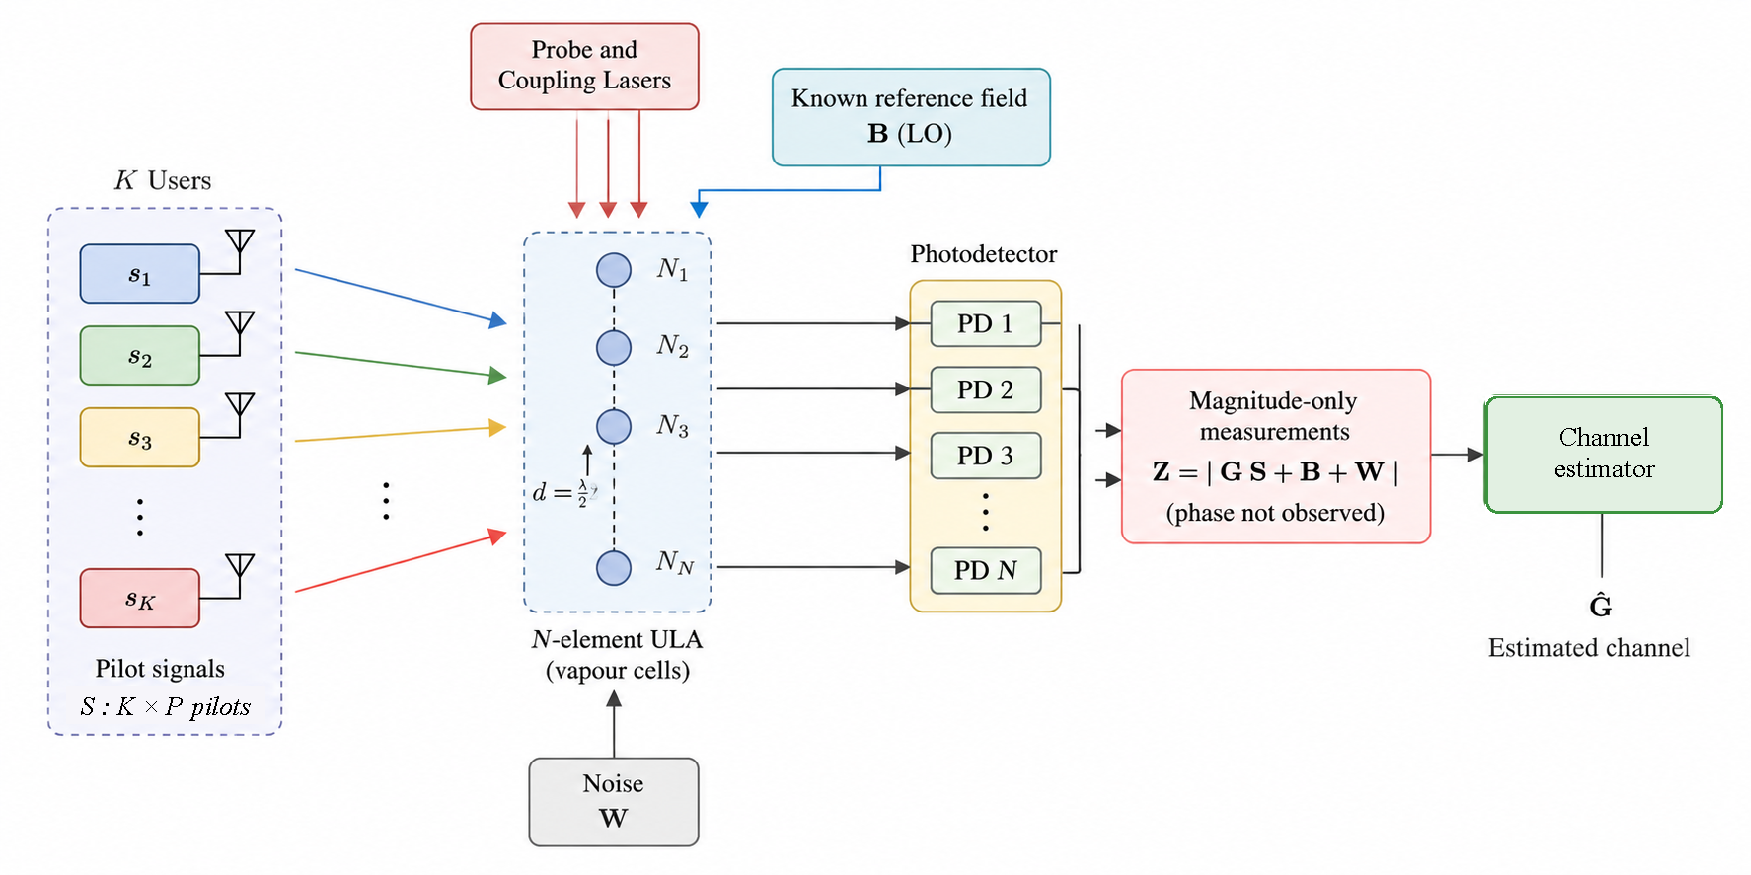
\includegraphics[width=\textwidth]{system_model.pdf}
\caption{Receiver model. $K$ users send known pilots to $N$ elements of a half-wavelength linear array. A known reference combines with the received field before magnitude measurement. The drawing shows the physical setup; the experiments model the resulting magnitudes, not the atomic dynamics or optical readout.}
\label{fig:system}
\end{figure*}
The array in Fig.~\ref{fig:system} receives $P$ pilots from $K$ users:
\begin{equation}
 Z=|GS+B+W|,\qquad W_{np}\sim\CN(0,v).
 \label{eq:model}
\end{equation}
Here $G\in\mathbb C^{N\times K}$ is the unknown channel, $S\in\mathbb C^{K\times P}$ contains the known pilots, and $B$ is the known reference. Magnitude acts on each entry. The noise samples are independent, with variance $v/2$ in each real component. Receiver gain is included in the signal scale.

For a half-wavelength linear array, user $k$ has channel
\begin{equation}
 g_{nk}=\sum_{\ell=1}^{L_k}\alpha_{\ell k}e^{-j\pi n\sin\theta_{\ell k}},
 \quad n=0,\ldots,N-1.
 \label{eq:channel}
\end{equation}
We draw $\alpha_{\ell k}\sim\CN(0,1/L_k)$ and angles uniformly on $(-\pi/2,\pi/2)$. Each user has expected channel power one; individual channels are not rescaled to equal energy. Pilots follow $\CN(0,1)$. The repeated reference and noise variance are
\begin{equation}
 B_{np}=10^{\mathrm{RSR}/20},\qquad v=K10^{-\mathrm{SNR}/10}.
\end{equation}
SNR uses the total user power. The reference-to-signal ratio (RSR) uses one user's power. Every estimator receives the correct reference and noise variance.

\subsection{How We Score a Channel Estimate}
For fixed variance, the Rician negative log-likelihood can be written, after removing terms independent of the channel, as
\begin{equation}
 \ell(z,\mu,v)=\frac{(z-|\mu|)^2}{v}-\log I_{0e}(2z|\mu|/v),
 \label{eq:loss}
\end{equation}
where $\mu=g^Ts+b$ and $I_{0e}(x)=e^{-x}I_0(x)$ is a scaled Bessel function. A lower loss means that the estimate better explains the noisy observations. Scaled functions avoid numerical overflow. If variance is also estimated, the omitted $\log v$ term must be restored.

A reference can reveal channel phase, but only with a suitable pilot/reference design. Without a reference, rotating the whole channel leaves every magnitude unchanged. An unknown reference phase also prevents recovery of absolute channel phase. For an unrestricted channel row, a full-rank real magnitude Jacobian gives local recovery and requires at least $P\ge2K$ pilots~\cite{gao2018}. This does not prove unique recovery over all possible channels. The supplement gives the Jacobian and Rician information calculation. The Cram\'er--Rao curves used later describe local limits under unbiasedness assumptions~\cite{stoica1998}; they are not absolute error bounds for our biased filters.

\section{Measurement Updates and Spatial Filtering}
\subsection{Exact EM Update}
EM alternates between estimating the missing complex field and updating the channel. For $M=GS+B$ and $\kappa=2Z|M|/v$, these steps are
\begin{align}
 Q&=Z\odot\frac{I_1(\kappa)}{I_0(\kappa)}\odot\frac{M}{|M|},\nonumber\\
 G_{\rm EM}&=(Q-B)S^H(SS^H)^{-1}.
 \label{eq:em}
\end{align}
The products and ratios in the first line act entry by entry, with value zero at $M=0$. The second line uses a linear solve and requires a full-row-rank pilot matrix. This is also a likelihood-gradient step scaled by the pilot Gram matrix $SS^H$.

The learned and direct-EM methods use the same spectral starting estimate. It comes from the leading eigenvector of a pilot/reference matrix weighted by the measured magnitudes. Only fitting pilots enter this step. The algebraic recovery method in Section~\ref{sec:receiver} provides a different starting point. Exact initialization formulas are in the supplement.

\subsection{Hard and Smooth Hankel Filters}
Let $q=\lceil N/2\rceil$, $m=N-q+1$, and define
\begin{equation}
 [\HH(g)]_{ij}=g_{i+j},\quad 0\le i<m,\quad0\le j<q.
\end{equation}
A channel with $L$ distinct spatial frequencies has Hankel rank at most $\min(L,m,q)$. The inverse map $\HH^\dagger$ averages entries on each antidiagonal. A hard filter keeps the largest $r$ singular components, then averages these entries. Repeating this operation gives Cadzow filtering.

Our classical Hankel-structured GS (HS-GS) control filters after each EM update. It selects a shared user rank using 70\% of the pilots for fitting and 30\% for validation, then restarts on all pilots. The default budgets are 25 updates per candidate, 100 final updates and four filtering sweeps per update. Rank $q$ allows filtering to be skipped. We call squared-amplitude-error selection HS-amplitude and Rician-loss selection HS-Rician.

A smooth filter instead changes each singular value by
\begin{equation}
 \widehat\sigma_i=\frac{\sigma_i^3}{\sigma_i^2+\tau^2}.
 \label{eq:shrink}
\end{equation}
Larger $\tau$ removes more of the smaller components; $\tau=0$ leaves them unchanged. A classical control selects $\tau$ from a small validation grid. OptShrink uses weights estimated from the remaining spectrum~\cite{nadakuditi2014}. We test offline-selected and per-block rank-selected versions in the earlier studies. Their complete searches, costs and numerical rules are given in the supplement.

\section{A Small Network That Chooses the Filter}
\subsection{Ten Estimation Stages}
Each learned start has ten stages. Stage $t$ first takes a relaxed EM step:
\begin{equation}
 G_{\rm dc}=G+\gamma_t(G_{\rm EM}-G),\qquad
 \gamma_t=2\sigmoid(a_t).
\end{equation}
The ten learned $a_t$ begin at $\gamma_t=1$. For user $k$, set $H_k=\HH(g_{{\rm dc},k})$, $s_H=\|H_k\|_F/\sqrt q$, and $p_i=\sigma_i/\sum_j\sigma_j$. A shared network with layer sizes 8--16--2 and SiLU activation receives
\begin{align}
 f_1&=\exp(-\textstyle\sum_i p_i\log p_i)/q,\quad f_2=p_1,\nonumber\\
 f_3&=\textstyle\sum_{i=q-\lceil q/2\rceil+1}^q p_i,\nonumber\\
 f_4&=\log\!\left(1+\operatorname{mean}[(Z-|G_{\rm dc}S+B|)^2]/v\right),\nonumber\\
 f_{5,k}&=\log\!\left(1+v\tr[(SS^H)^{-1}]/(K\widehat p_k)\right),
 \label{eq:features}
\end{align}
and $P/(2K)$, $\log q$, $(t+1)/10$, where $\widehat p_k=\|g_{{\rm dc},k}\|_2^2/N$. In plain terms, these inputs describe the spread of singular values, the measurement mismatch, the noise level, pilot support, array size and stage number. None uses the true channel or path count.

The two network outputs $(u,w)$ give
\begin{equation}
 \tau=s_H[0.001+\softplus(u)],\qquad\beta=\sigmoid(w).
\end{equation}
The parameter $\tau$ sets how strongly the singular values shrink. The parameter $\beta$ sets how much of that filtered result is used:
\begin{align}
 F_\tau(H)&=H-\tau^2H(H^HH+\tau^2I)^{-1},\label{eq:solve}\\
 g_k^{t+1}&=g_{{\rm dc},k}+\beta_{t,k}
 [\HH^\dagger F_{\tau_{t,k}}(H_k)-g_{{\rm dc},k}].
\end{align}
Thus $\beta$ near zero keeps the EM result, while $\beta$ near one uses the full filter correction. The solve implements~\eqref{eq:shrink}; training differentiates through it. The network has 178 parameters, and the ten EM step sizes give 188 in total. The inputs still require singular values. Neither $\tau$ nor $\beta$ is a physical path-count estimate.

\subsection{Training Without Knowing the True Channel}
Each training example contains 39 simulated pilot observations. A changing random split gives 30 input columns $A$ and nine withheld columns $V$. They have independent measurement noise; the pilot matrix is screened jointly before splitting. The network sees only $A$, produces $\widehat G_A$, and is trained to predict $V$ through
\begin{equation}
 \mathcal L_{\rm hold}=\frac{1}{N|V|}\sum_{n,p\in V}
 \ell\big(Z_{np},[\widehat G_A S_V+B_V]_{np},v\big).
\end{equation}
An adjustment to $\tau$ or $\beta$ is rewarded when it lowers this prediction loss. The computer sends that loss backward through the ten stages to update the network weights. The true channel is never the training target. At use time, all 30 available pilots enter the estimate, and the network weights stay fixed.

Training uses 16,384 examples, 2,048 separate validation examples, 20 epochs, batch size 32 and Adam learning rate $10^{-3}$. Half the examples have independent 3--7 paths per user; the rest use shared path counts $2,4,8,12,16$. Seven SNRs from $-10$ to 20~dB and three reference levels define 126 validation groups. The checkpoint with the lowest equally weighted withheld loss is selected, including the untrained checkpoint. Three training runs use the same data population. Training uses single precision; final testing uses double precision.

A fixed trained schedule learns only a step size, threshold and mixing value for each stage: 30 parameters. Its values do not change with the input, apart from the stated signal-scale normalization. It uses the same data, splits and training budget as the adaptive network. The complete receiver stores one model of each kind, for 218 neural parameters. Earlier 21-input-pilot and alternative-training studies remain separate in the supplement.

\subsection{What the Update Bounds Mean}
For fixed $\tau$, the smooth filter satisfies
\begin{equation}
 \|F_\tau(H)\|_F\le\|H\|_F,\qquad
 \|F_\tau(H)-H\|_F\le\sqrt q\,\tau/2.
 \label{eq:bound}
\end{equation}
The second inequality follows by maximizing $\sigma\tau^2/(\sigma^2+\tau^2)$. After antidiagonal averaging, the correction has a corresponding bound scaled by $\beta$. This limits how much the filter changes the estimate; it does not prove that channel error decreases. Relaxed EM also decreases its quadratic fitting objective for $0\le\gamma_t\le2$, but the later filter can undo that decrease. Full-estimator convergence and guaranteed BER improvement do not follow. The supplement gives the proofs and numerical details.

\section{Choosing the Start and Checking the Result}
\label{sec:receiver}
The receiver uses the adaptive model at ordinary SNR and a fixed trained schedule at higher SNR. It can then try a separate recovery step. All choices use the measured pilots, known reference, supplied noise variance and stored settings. They never use the true channel or test error.

\subsection{Learned and Fixed Schedules}
Define $s=10\log_{10}(K/v)$ and $r=10\log_{10}\operatorname{mean}|B|^2$. Under our normalization these equal the nominal SNR and RSR. They do not estimate the power of an individual channel. The adaptive model is used through 30~dB; the fixed schedule is used above 30~dB. Only one model is run for each block.

At $s\le20$~dB, the adaptive output is returned directly. Above 20~dB, a stored reference/SNR table selects 0, 10, 20 or 40 extra EM updates and a final noise-based filter. This filter uses $\beta=1$ and
\begin{equation}
 \tau_k=c\sqrt{2v\operatorname{Re}[(SS^H)^{-1}]_{kk}\max(m,q)},
 \label{eq:finaltau}
\end{equation}
where $c\in\{0,2,4\}$ and $c=0$ skips the filter. This is a chosen noise scale, not an exact error covariance. The table uses the nearest tested reference and SNR, with lower values at a tie. All entries, boundary tolerances and off-grid rules are in the supplement.

The strong-reference filter stays active above 40~dB. Removing it at that point caused an earlier jump in error. Other changes between table entries remain. Let $G_0$ be the complete estimate after the chosen model, extra EM and final filter.

\subsection{When to Try Another Starting Estimate}
The added recovery check applies only to the nearest-reference 5~dB range and $s>30$~dB. It measures the mismatch at each antenna:
\begin{equation}
 R_n=\frac{2}{Pv}\sum_p\bigl(Z_{np}-|[G_0S+B]_{np}|\bigr)^2.
 \label{eq:gate}
\end{equation}
If $\max_nR_n>2$, the receiver tries an algebraic starting estimate. The maximum helps detect one poorly fitted antenna that an average might hide. This residual is a useful check, not a probability that the channel is wrong. If the check does not apply or does not trigger, the result stays exactly $G_0$.

For a repeated, nonzero reference $B_{np}=b_n$, set $c_n=g_n/b_n$ and
\begin{equation}
 y_{np}=\frac{Z_{np}^2-v}{|b_n|^2}-1.
\end{equation}
Subtracting the known noise power gives
\begin{equation}
 \mathbb E[y_{np}\mid G,S,B]
 =2\operatorname{Re}(c_n^Ts_p)+|c_n^Ts_p|^2.
 \label{eq:intensity}
\end{equation}
For $K=3$, this is linear in 15 real coefficients: six channel components and nine extra coefficients for the quadratic terms. The real $P\times15$ design matrix $D$ has columns
\begin{equation}
 2\operatorname{Re}s_i,\;-2\operatorname{Im}s_i,\;|s_i|^2,\;
 2\operatorname{Re}(s_is_j^*),\;-2\operatorname{Im}(s_is_j^*)
\end{equation}
for each user $i$ and pair $i<j$. One least-squares solve serves all antennas. The six linear coefficients recover $c_n$ and then $g_n=b_nc_n$. The quadratic coefficients are fitted freely; the solve does not force them to equal products of the recovered channel.

If $D$ has full column rank, the noiseless equations give the exact channel. With correct noise subtraction, this unfiltered linear estimate is conditionally unbiased. These statements do not extend to the later nonlinear steps. The implementation checks rank 15, condition number at most $10^8$ and finite values. Constant-magnitude pilots make three design columns identical up to scale, so this rank check rejects QPSK fitting pilots. Our experiments use Gaussian fitting pilots. The supplement gives the proof, noise variance and this design limitation.

\subsection{Refinement and Acceptance}
A valid algebraic estimate receives 20 exact EM updates and the same final filter as $G_0$. Call the result $G_{\rm alt}$. It replaces $G_0$ only if its average fitting loss satisfies
\begin{equation}
 \overline{\mathcal L}(G_{\rm alt})<
 \overline{\mathcal L}(G_0)-10^{-12}.
 \label{eq:accept}
\end{equation}
An invalid solve or a rejected alternative leaves $G_0$ unchanged. The whole channel is replaced together. This rule prevents an increase in computed fitting loss. It cannot guarantee lower channel error or BER.

The complete order is: run the selected model, apply its extra EM and final filter, check the residual, optionally compute the alternative, then compare losses. All steps count toward runtime. No extra online pilots or online weight training are used. The separate algebraic-plus-EM20 baseline tries the algebraic start everywhere; if that solve is invalid, it uses the spectral start plus 20 EM steps.

\section{How the Receiver Is Tested}
\label{sec:protocol}
\subsection{Separate Development and Test Data}
The final test uses $N=32$ antennas, $K=3$ users and $P=30$ fitting pilots. It crosses three reference levels (5, 12 and 20~dB), three path cases (two, four or independent 3--7 paths per user), and 17 SNRs:
\begin{equation*}
 \begin{gathered}
 \{0,5,10,15,20,22.5,25,27.5,30,32.5,\\
 35,37.5,40,42.5,45,50,60\}\ \mathrm{dB}.
 \end{gathered}
\end{equation*}
Each reference/path group has 128 independent channel/pilot/noise draws. The same draws are reused across SNR by changing the noise scale. Thus there are 153 settings and 19,584 test cases, but only 1,152 independent channel draws. All methods share observations. The three training runs are scored separately, not combined into one prediction. The simulator screens nearly coincident paths and nearly singular steering and pilot matrices as specified in the supplement. True channels are used only to score errors.

Before the final test, separate development and confirmation data select the new recovery rule. The candidates combine a mean or maximum residual, thresholds 2/4/8 and 10/20 extra EM steps. All 12 pass a separate runtime screen. Selection uses withheld pilot loss and known-symbol communication probes, not true-channel errors. Only the selected maximum/2/20 rule is checked on independent confirmation data. Its one-sided 95\% lower bound for loss improvement is 0.1987. Both methods have zero observed probe errors, which does not prove equal population BER. The selected rule is fixed before the final test is generated.

This confirmation applies to the new recovery check. The earlier extra-EM table was exploratory, and its earlier confirmation failed. We retain that fact and do not present the new check as confirmation of every inherited choice. Earlier classical and training studies use separate data; their results are not pooled into the final comparison.

\subsection{Fair Comparisons and BER}
All final methods receive the same 30 pilots, reference and noise variance. Controls include the previous hybrid, the earlier full repair, and adaptive, fixed-schedule and classical starts with the same 40 extra EM steps and final filter. Each start already has ten stages. The classical start uses fixed noise multiplier $c=1$ and mixing $\beta=1$, selected from 30 choices on the same validation data. Spectral EM100 uses the common starting estimate and 100 EM steps.

The angle-domain sparse/EM control uses the same Rician model. Its fixed table has 51 reference/SNR entries: 34 choose a sparse solver with 128 or 256 dictionary columns, while 17 choose direct EM100. It is therefore a sparse/EM combination. Full settings and selection records are included in the supplement. OptShrink was excluded before this final test because earlier p90 times were about 79--81~ms; its earlier comparisons remain separate. Published URformer is not reproduced.

Every estimated channel is passed to the same magnitude-domain detector:
\begin{equation}
 \widehat x=\arg\min_{x\in\mathcal Q^K}\sum_n
 \ell(z_n^{\rm d},\widehat g_n^Tx+b_n,v),
\end{equation}
where $\mathcal Q$ is unit-power QPSK. Each channel sends all 64 joint symbol vectors once, giving 384 bits per test case and 7,520,256 bits per training run. Data noise is independent of pilot noise. All estimators see the same data observations, which are unavailable during channel estimation. A detector given the true channel provides a reference curve only.

\subsection{Error Scores and Processing Time}
Normalized mean squared error (NMSE) divides squared channel error by channel energy. For each setting and method $a$, we use
\begin{equation}
 E_a=10\log_{10}\frac{\sum_i\|\widehat G_{a,i}-G_i\|_F^2}
 {\sum_i\|G_i\|_F^2}.
 \label{eq:nmse}
\end{equation}
The main score gives each of the 153 settings equal weight, then averages scores from the three training runs. Pooled NMSE instead combines all squared errors and channel energies before taking their ratio. These scores can rank methods differently. BER is the fraction of decoded bits that are wrong. The grid has 108 settings above 20~dB, so it does not represent a typical deployment mix.

We use 20,000 paired bootstrap draws: repeated resampling of the independent channel draws to measure uncertainty. Resampling stays within each of the nine reference/path groups and preserves shared draws across SNR, methods and training runs. Four main comparisons cover NMSE and BER against the previous hybrid and full repair; their 95\% familywise intervals use Bonferroni adjustment. Other intervals are descriptive. They do not measure variation from new training populations, and zero observed errors do not prove zero true BER.

Two separate timing runs measure complete processing of one channel block on one CPU thread in double precision. Both include initialization, all filters, checks, solves and extra EM, including rejected alternatives. They exclude training, model loading, preloaded constants, data generation and BER decoding. We require the 90th-percentile time (p90) to be at most 10.74~ms over both the full grid and weak-reference target range in both runs. This means 90\% of measured calls fall below that value; it is not a deadline for every call. Neither timing run is repeated to obtain a pass. The supplement gives call counts, software details and both runs.

\section{Results}
\subsection{Earlier Tests: When Spatial Filtering Helps}
\begin{figure*}[!t]
\centering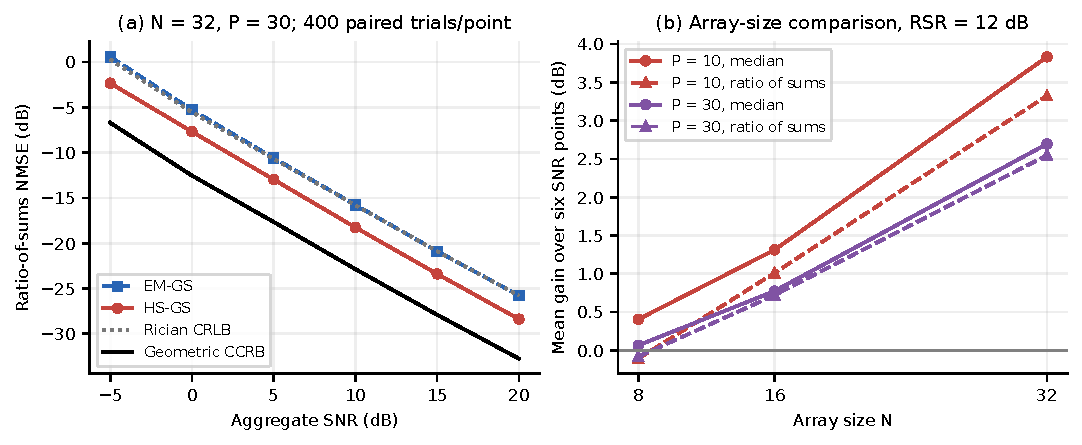
\includegraphics[width=\textwidth]{classical_array.pdf}
\caption{Earlier classical study. Left: channel error and information references for 32 antennas and 30 pilots. Right: gain from HS-amplitude filtering as array size grows. HS-GS uses four filtering sweeps. Solid lines average paired-median gains over six SNRs; dashed lines combine squared errors within each setting before averaging gains. These are separate tests from Table~\ref{tab:reliability-main}.}
\label{fig:classical}
\end{figure*}
The earlier array study uses 400 shared channel draws per setting, three users, 10 or 30 pilots and RSR 12~dB. With 32 antennas and 30 pilots, hard Hankel filtering improves the paired-median error over EM-GS by 2.54--2.97~dB across six SNRs (Fig.~\ref{fig:classical}). Averaging the pilot counts and SNRs gives gains of 0.236, 1.044 and 3.264~dB for 8, 16 and 32 antennas. Larger arrays provide more samples of the same spatial paths. The information curves describe local unbiased-estimation limits, not a guaranteed gain for the filters.

To describe how strongly the channel is concentrated in a few spatial components, define the effective rank~\cite{royvetterli2007}
\begin{equation}
 r_{\rm eff}=\exp(-\textstyle\sum_i p_i\log p_i),\qquad \rho=r_{\rm eff}/q.
\end{equation}
A low value means a few singular values carry most of the channel. Here $\rho$ is calculated from the true channel for analysis; the receiver cannot use it.
\begin{figure}[!t]
\centering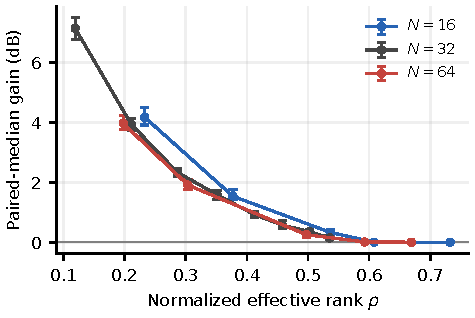
\includegraphics[width=\columnwidth]{effective_rank.pdf}
\caption{Earlier structure test. Hard-filter gain falls as more spatial components become important. The horizontal axis uses the true channel and cannot serve as an online switching rule. Bars show pointwise paired-bootstrap intervals. The arrays use 20 pilots, RSR 10~dB and the same random-SNR distribution.}
\label{fig:rank}
\end{figure}
Figure~\ref{fig:rank} shows that hard filtering generally helps less as $\rho$ rises. At $N=32$ and $\rho=0.536$, the median gain is only 0.141~dB. At $N=16$, $L=14$ and $\rho=0.732$, forcing rank seven loses 0.154~dB. A value near one-half marks a small gain in this test, not a general threshold. At 32 antennas, 14 paths and SNR 0~dB, even selected-rank filtering is worse than EM-GS in 47.75\% of draws. Smooth classical filtering improves on four hard sweeps by 0.914--1.413~dB in the tested 0~dB cases. Thus learning is not required to improve hard truncation, and more filtering is not always better.

\subsection{What the Earlier Learned Study Shows}
A separate 126-setting study tests the original models trained with 21 input pilots. On its 4,032 main channel draws, the 188-parameter controller improves mean-setting NMSE by 1.835~dB over the fixed schedule and 1.967~dB over a matched recurrent control, with adjusted intervals $[1.805,1.871]$ and $[1.932,2.006]$~dB. The recurrent control is inspired by NA-ALISTA, not a reproduction of that published method. Per-block rank-selected OptShrink is 0.452~dB better than the controller on this score, but much slower. These results support the adaptive component on that earlier test; they are not measurements of the final receiver. The supplement preserves all earlier training studies and their limits.

\subsection{Final Channel Error and BER}
\begin{table*}[!t]
\centering
\caption{Final comparison across 153 test settings. Lower values are better. Time is the slower result from two separate runs.}
\label{tab:reliability-main}
\small
\setlength{\tabcolsep}{4pt}
\begin{tabular}{lrrrrr}
\toprule
Method & \shortstack{Mean-setting\\NMSE (dB)} & \shortstack{Pooled linear\\NMSE} & BER (\%) & \shortstack{Full-grid\\p90 (ms)} & \shortstack{Target-range\\p90 (ms)} \\
\midrule
Proposed receiver & -38.620 & 0.00897384 & 0.522496 & 7.254 & 7.031 \\
Previous hybrid & -38.113 & 0.00900482 & 0.522496 & 7.148 & 6.809 \\
Earlier full repair & -37.858 & 0.00903694 & 0.522571 & 14.690 & 14.858 \\
Adaptive start + EM40 & -35.691 & 0.02637969 & 0.808204 & 9.040 & 8.704 \\
Fixed schedule + EM40 & -36.482 & 0.02658368 & 0.813718 & 7.103 & 6.745 \\
Classical start + EM40 & -32.005 & 0.02744311 & 0.809387 & 7.142 & 6.802 \\
Spectral EM100 & -30.562 & 0.02839215 & 0.828828 & 8.835 & 8.752 \\
Compact sparse/EM & -31.895 & 0.00868525 & 0.489159 & 9.516 & 8.756 \\
Algebraic start + EM20 & -36.534 & 0.02788204 & 0.835676 & 3.101 & 2.747 \\
\bottomrule
\end{tabular}
\par\vspace{2pt}
\begin{minipage}{0.98\textwidth}\footnotesize Learned rows average scores from three training runs, not channel predictions. Mean-setting NMSE gives each setting equal weight; pooled NMSE combines squared errors before forming the ratio. EM40 means 40 extra EM updates. The target range is RSR 5~dB and SNR $>30$~dB (24 settings). The 10.74~ms limit applies to p90 in both ranges and runs, not to every call. Sparse/EM has the best pooled NMSE and overall BER.\end{minipage}
\end{table*}

Table~\ref{tab:reliability-main} gives the new comparison on shared test observations. The proposed receiver improves mean-setting NMSE by 0.507~dB over the previous hybrid, with adjusted interval $[0.338,0.652]$~dB. It improves by 0.762~dB over the full repair, with interval $[0.231,0.878]$~dB. Gains over the previous hybrid are similar across the three training runs: 0.497, 0.504 and 0.521~dB. Gains over the full repair vary more: 0.361, 0.114 and 1.810~dB.

The proposed and previous receivers have the same observed overall BER, 0.522496\%. The full repair makes 17 more bit errors across the three runs, all in one run, but the adjusted interval includes zero improvement. We therefore do not claim a proven BER gain over either main comparison. Sparse/EM remains better in overall BER (0.489159\%) and pooled NMSE (0.008685 versus 0.008974). The best average dB score does not mean the best result under every measure.

\begin{figure*}[!t]
\centering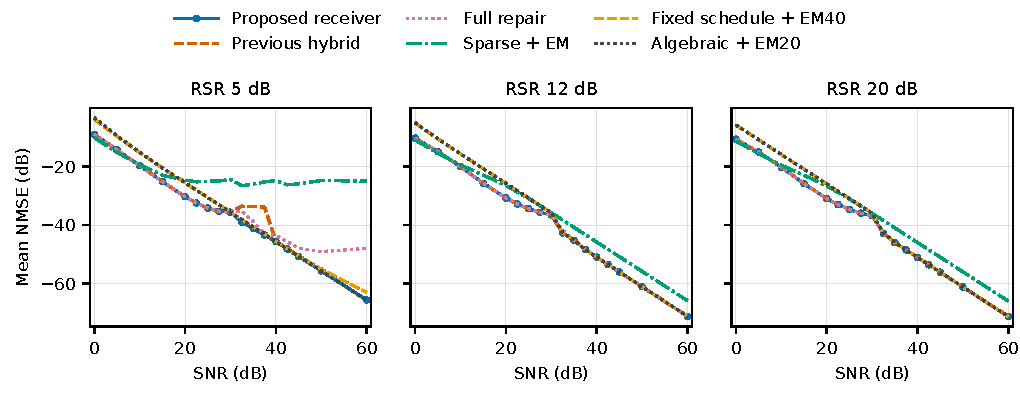
\includegraphics[width=\textwidth]{reliability_nmse.pdf}
\caption{Final channel-error comparison. Each point averages the three path-setting scores. Learned methods also average the scores from three training runs, not their channel estimates. All methods share observations. A fixed schedule and algebraic recovery both give strong high-SNR results.}
\label{fig:reliability-nmse}
\end{figure*}
\begin{figure*}[!t]
\centering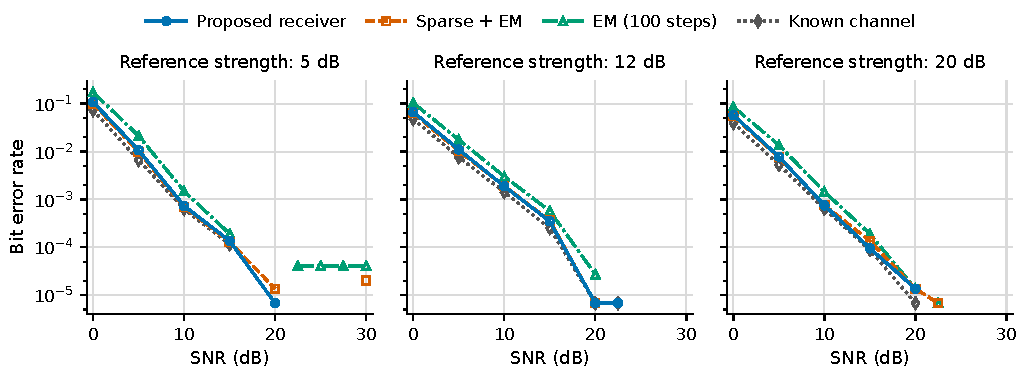
\includegraphics[width=\textwidth]{reliability_ber.pdf}
\caption{Bit error rate from 0 to 30~dB, averaged over the three path settings. All methods use the same data and detector. ``Known channel'' gives the detector the true channel. Points with no observed errors are omitted from the log scale, and lines break at those points. The supplement shows the full 0--60~dB range.}
\label{fig:reliability-ber}
\end{figure*}
Figure~\ref{fig:reliability-nmse} shows the full SNR range. Figure~\ref{fig:reliability-ber} focuses on the range where most bit errors occur. Zero observed errors cannot be drawn on a logarithmic axis and do not prove zero true BER. High-SNR results remain in Table~\ref{tab:reliability-regions} and the full-range supplementary plot.

\subsection{Where the Recovery Check Helps}
\begin{table*}[!t]
\centering
\caption{Results in three SNR ranges on the same final test data.}
\label{tab:reliability-regions}
\small
\setlength{\tabcolsep}{4pt}
\begin{tabular}{llrrrrr}
\toprule
Region & Metric & Proposed & \shortstack{Previous\\hybrid} & Full repair & Sparse/EM & Algebraic20 \\
\midrule
Ordinary (45) & dB & -20.242 & -20.242 & -20.242 & -18.964 & -15.470 \\
 & BER (\%) & 1.776440 & 1.776440 & 1.776440 & 1.662191 & 2.841254 \\
Weak target (24) & dB & -48.644 & -45.411 & -43.893 & -25.607 & -48.457 \\
 & BER (\%) & 0.000000 & 0.000000 & 0.000480 & 0.001441 & 0.000000 \\
High SNR (45) & dB & -56.744 & -56.512 & -54.638 & -44.052 & -56.754 \\
 & BER (\%) & 0.000000 & 0.000000 & 0.000196 & 0.000633 & 0.000000 \\
\bottomrule
\end{tabular}
\par\vspace{2pt}
\begin{minipage}{0.98\textwidth}\footnotesize Ordinary: SNR $\leq20$~dB, all references. Weak target: RSR 5~dB and SNR $>30$~dB. High SNR: SNR $\geq40$~dB, all references. These ranges overlap; their comparisons are descriptive. Zero BER means no observed bit errors, not proof of zero true error. The first three methods give exactly the same estimates in the ordinary range.\end{minipage}
\end{table*}

The recovery check targets reference 5~dB and SNR above 30~dB: 24 settings. Here the mean NMSE is $-48.644$~dB. The gain is 3.232~dB over the previous hybrid, with descriptive interval $[2.249,3.966]$~dB, and 4.750~dB over the full repair, with interval $[1.836,5.326]$~dB. The check triggers on about 26.7--27.0\% of target cases across training runs. Every triggered alternative is accepted in this test, and none has an invalid design.

Fifteen of the 153 setting means improve over the previous hybrid; the rest are equal. No setting mean is worse, though individual channel errors can be worse. All outputs at SNR at most 20~dB, and all cases outside the new check, remain exactly unchanged. Both methods have zero observed bit errors in the target range. The large channel-error gain therefore gives no measured BER gain there.

The proposed receiver is worse than the full repair in 32 setting means. Eight pointwise intervals exclude zero; these are descriptive comparisons, not simultaneous findings across all settings. The largest loss is 0.701~dB at two paths, reference 20~dB and SNR 32.5~dB, outside the new check. At strong references and SNR at least 40~dB, mean NMSE is $-58.555$~dB versus $-58.558$~dB for the full repair. We retain these losses rather than retune on the final test.

Algebraic-plus-EM20 is close to the proposed receiver in the target range ($-48.457$~dB) and is the fastest full pipeline in the table. Across the full grid, however, its BER is 0.835676\%. This supports combining the methods while showing that learning is not needed for accurate high-SNR recovery. Sparse/EM's BER advantage is concentrated in ordinary-SNR operation, which the new check preserves rather than improves.

\subsection{Runtime and Remaining Limits}
The proposed receiver passes both required p90 checks in both timing runs. Full-grid times are 4.282 and 7.254~ms; target-range times are 4.162 and 7.031~ms. The table reports the slower run. The second run is also slower for the baselines. The full repair passes in the first but fails in the second, at 14.690~ms overall and 14.858~ms in the target range.

The proposed receiver's maximum times are 5.225 and 22.276~ms. One of 1,377 calls in the second run exceeds 10.74~ms, even though its recovery check does not trigger. The measurements do not identify the cause. Passing the p90 target is therefore different from meeting a deadline on every call.

Earlier tests found that strong learned filtering can cause bias when noise is very small, and that wrong noise or reference-phase inputs can increase error. The final receiver has not been validated under these errors. Correct reference phase, correct variance, Gaussian fitting pilots and the stated linear-array model remain assumptions. Tests on atomic hardware, other user counts, other array shapes and coded communication links remain future work.

\section{Conclusion}
The network learns how much spatial filtering to apply from the current estimate and observations. The recovery step addresses a different problem: a poor starting estimate. It tries an algebraic alternative and keeps it only when the fitting loss improves. The receiver combines these parts according to the supplied noise and reference levels.

On the final shared test, this design improves channel error over the previous hybrid, preserves its observed BER, and meets the 10.74~ms p90 target in both timing runs. It keeps the ordinary-SNR output unchanged and improves recovery at weak references and high SNR. Sparse/EM still has better overall BER and pooled NMSE. The result supports a useful combination of learned and classical methods, with clear limits.

The source package includes all settings, numerical summaries and five checks covering selection, predictions, BER, statistics and timing. The supplement retains the earlier studies and additional method details. Large raw simulation files and trained weights are not included in this manuscript package; a permanent public code/data archive remains to be assigned. The three training runs share one data population. A matched URformer comparison, calibration-error tests and new training populations would strengthen the evidence.

\section*{Acknowledgment}
OpenAI's ChatGPT/Codex assisted with writing, experiment-code development and figure scripts. The author is responsible for checking the content and final submission.
\IEEEtriggeratref{20}
\bibliographystyle{IEEEtran}
\bibliography{references}
\end{document}
